\documentclass[review,5p,twocolumn,sort&compress,times]{elsarticle}

\usepackage{lineno}
% \usepackage{hyperref}

%%%%%% SYMBOLES %%%%%
\usepackage{tipa}	% pour avoir l'accent concave
\usepackage{lmodern}	% pour les guillemets
\usepackage{nth}	% pour ^th près des chiffres

%%%%%% EQUATION %%%%%%
\usepackage{amssymb}
\usepackage{amsmath}
\usepackage{fancybox}
\usepackage{xfrac}	% fraction de type "1/4"
\usepackage[fleqn]{cases}	% système équation
\usepackage[overload]{empheq}
\usepackage{bm}		% pour mettre en gras .
\usepackage{units} 	% x/y barre latérale pour les fractions
%\usepackage{split}

%%%%%% FIGURE %%%%%%
\usepackage{graphicx}	% insérer des graphiques
\usepackage{float}	% utiliser H dans les figures
\usepackage{subcaption}


%%%%%% TABLEAUX %%%%%%
\usepackage{array,multirow,makecell}
\usepackage[table,xcdraw]{xcolor} % pour avoir des lignes colorées dans les tableau
\usepackage{hhline}	% pour les lignes horizontales
\usepackage{tabularx} % permet itemize dans les cellules
\usepackage{booktabs}

\newcolumntype{L}[1]{>{\raggedright\let\newline\\\arraybackslash\hspace{0pt}}m{#1}}
\newcolumntype{C}[1]{>{\centering\let\newline\\\arraybackslash\hspace{0pt}}m{#1}}
\newcolumntype{R}[1]{>{\raggedleft\let\newline\\\arraybackslash\hspace{0pt}}m{#1}}

%%%%%%%%%%%%%%%%%%%%%
\usepackage{url}	% gérer les adresses www.

\newcommand{\ml}[1]{\textcolor{red}{ML : #1}}
\modulolinenumbers[5]

\begin{document}

\begin{frontmatter}

\title{Road traffic sound level estimation from realistic urban sound mixtures by Non-negative Matrix Factorization}

\author[ifsttar]{Jean-R\'emy Gloaguen\corref{cor1}}
\ead{jean-remy.gloaguen@ifsttar.fr}
\author[ifsttar]{Arnaud Can}
\author[ls2n]{Mathieu Lagrange}
\author[ls2n]{Jean-Fran\c cois Petiot}

\cortext[cor1]{Corresponding author}
\address[ifsttar]{Ifsttar Centre de Nantes, UMRAE, All\'ee des Ponts et Chauss\'es, 44344 Bouguenais, France}
\address[ls2n]{LS2N, 1 rue de No\"e, 44331 Nantes, France}

\begin{abstract}

Experimental acoustic sensor networks are currently tested in large cities, and appear more and more as a useful tool to enrich modeled road traffic noise maps through data assimilation techniques. One challenge is to be able to isolate from the measured sound mixtures acoustic quantities of interest such as the  sound level of road traffic. This task is anything but trivial because of the multiple sound sources that overlap within urban sound mixtures.

In this paper, a Non-negative Matrix Factorization (NMF) framework is developed to estimate road traffic noise levels within urban sound scenes. To evaluate the performance of the proposed approach, a synthetic corpus of sound scenes is designed to cover most common soundscape settings. The realism of the produced scenes is validated through a perceptual test, forming a protocol that both reproduces the sensor network outputs, and in which the actual occurrence and sound level of each source is known.

Several variants of NMF are tested. The threshold initialized NMF appears to be the most relibale approach, allowing road traffic noise level estimation with average errors of 1.3 dB over the tested corpus of sound scenes.

\end{abstract}

\begin{keyword}
non-negative matrix factorization \sep urban sound environment \sep road traffic sound level estimation
\end{keyword}

\end{frontmatter}

\linenumbers

\section{Introduction}

In response to the growing demand from urban dwellers for a better environment, noise mapping has been recommended as a tool to tackle noise pollution. The enactment of the European Directive 2002/EC/49 makes such maps mandatory to cities over 100 000 inhabitants. Those maps play an important informative role, establishing the distribution of the sound levels all over the cities as well as the estimation of the number of city dwellers exposed to high sound level ($>$ 55 dB(A)) \cite{nugent2014noise}. Road traffic concentrates particular attention as it is the main urban source of noise annoyance. Road traffic noise maps are typically built from data collection that consist of traffic data collected on the main roads (flow rates, mean speeds and heavy vehicle ratio) and urban geographic data (building heights and location, topology, ground surfaces, etc.). Follows sound emission and sound propagation computational techniques, resulting in the production of the two indicators equivalent A-weighted sound levels, $L_{DEN}$ (\textit{Day-Evening-Night}) and $L_N$ (\textit{Night}) \cite{kephalopoulos2012common}. This procedure also enables drawing up action plans to reduce the noise exposure. Despite their unanimously recognized interest, noise maps suffer some limitations. The computing cost required to produce noise maps at the city scale calls simplifications of the numerical tools and the simulation models that both generate uncertainties \cite{van_leeuwen_noise_2015}. Data collection is itself also a vector of uncertainty. Moreover, the produced aggregated indicators do not model the sound levels evolution due to the traffic variations throughout the day.

Noise measurements are thus increasingly used in addition to simulation to describe urban noise environments. Several measurement set-ups have been proposed in the last years, including  mobile measurements with high quality microphones \cite{manvell2004sadmam, can2014measurement}, participative sensing through dedicated smartphone applications \cite{picaut:halshs-01565214, ventura2017evaluation}, or the development of fixed-sensor networks. In this latter case, the sensor networks can be based either on high-quality sensors as in \cite{mietlicki2012innovative, maijala2018environmental}, or low-cost sensors as in the DYNAMAP project \cite{dynamap_2016} or the CENSE project \cite{picaut2017characterization}. The costs and benefits of each protocol are discussed. Mobile and participatory measures increase spatial coverage at low cost, but lack temporal representativeness. Fixed networks are very reliable for measuring sound levels temporal variations, but allow only a small spatial coverage of the network. In addition, the low-cost sensors enable a wider deployment, but at the cost of increased uncertainties, the most extreme example being smartphone applications.

\begin{figure}[t]
\centering
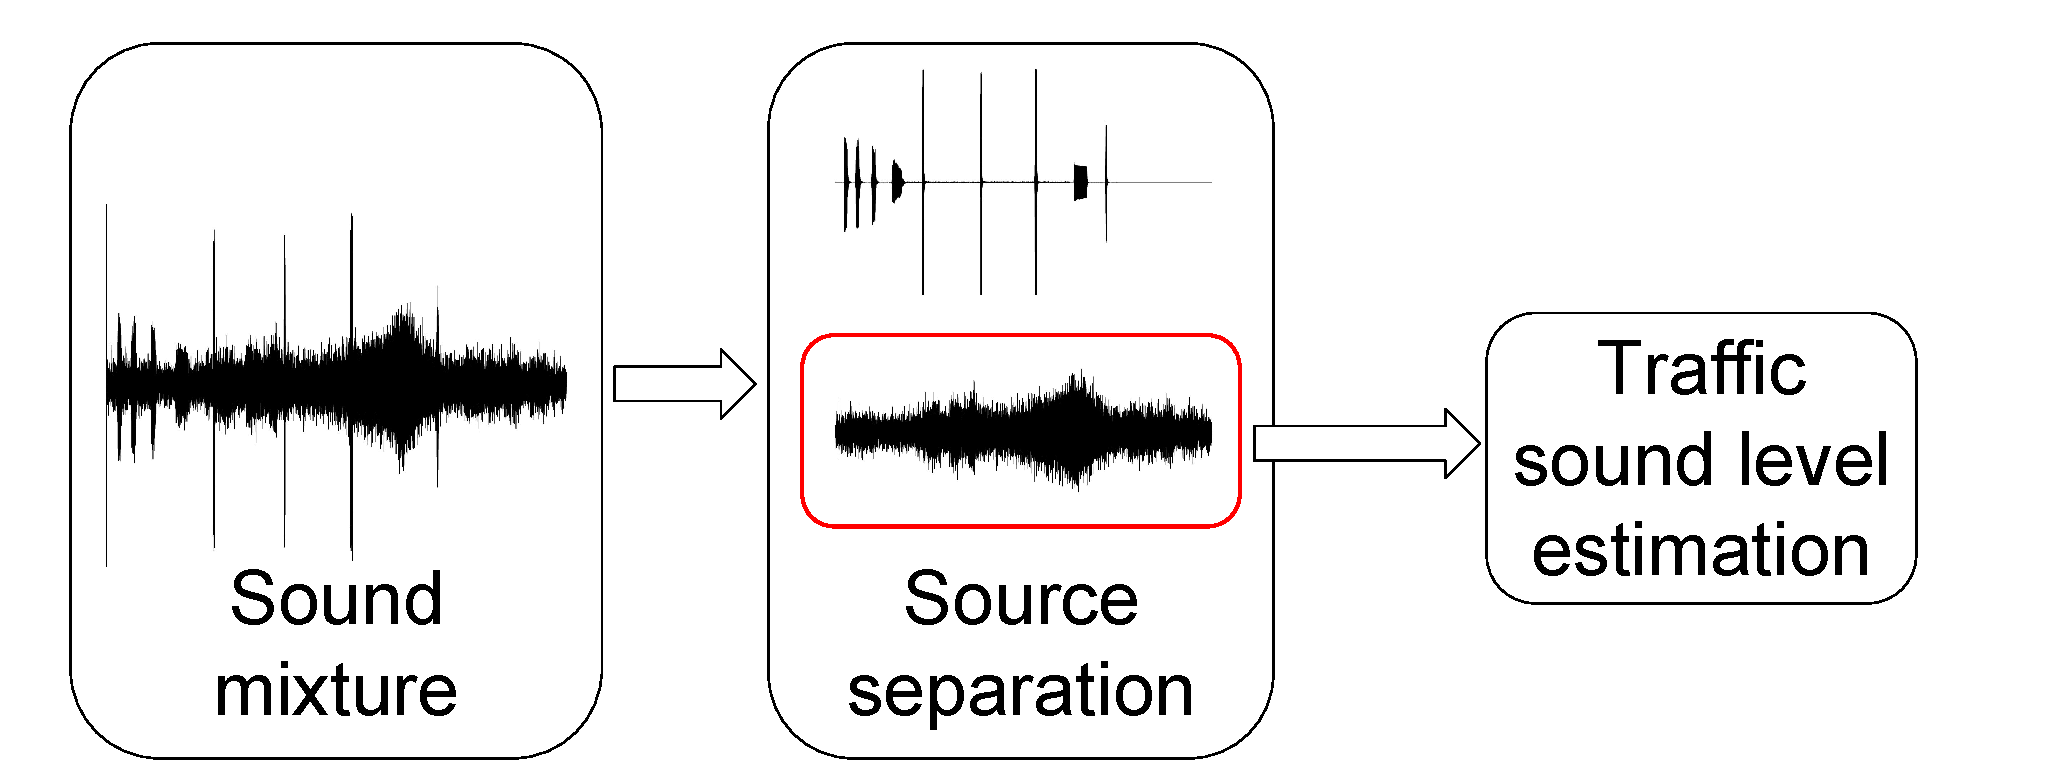
\includegraphics[width=.9\linewidth]{figures/bloc_diagram_source_separation.pdf}
\caption{Block diagram of the blind source separation model}
\label{fig:source_separation}
\end{figure}

All these measurement protocols allows the combination of measures and predictions to improve the accuracy of the produced noise maps. Traffic noise maps and measurements were compared on restrictive areas in \cite{lefebvre2017traffic} and \cite{mioduszewski2011noise}. Wei et al. \cite{wei_dynamic_2016} modify the acoustical parameters of the simulation thanks to noise measurements, while  Mallet et al. \cite{ventura2017estimation} call for data assimilation techniques between models and measurements to reduce the uncertainty of the produced noise maps. However, these works make the implicit assumption that the noise measurements consist mainly of road traffic. In the aim to improve road traffic noise maps, the use of measurements has first to deal with the challenge to estimate correctly the road traffic sound level.
Even if road traffic is predominant on many urban areas, urban sound environments are composed of many different overlapping sound sources (passing cars, voices, footsteps, car horn, whistling birds \dots), what makes the task of estimating correctly the traffic sound level within an urban sound mixture not trivial.

Many works have dealt with the detection \cite{luitel2016sound} or the recognition \cite{defreville_automatic_2006} of sound events in environmental sound scenes. In these cases, a two-step scheme is followed where audio samples are described with a set of features (Mel Frequency Cepstral Coefficient, MPEG-7 descriptors \dots) and classified them with the help of a classifiers (Gaussian Mixtures Models, Artificial Neural Network \dots) \cite{chu2008environmental, cowling_comparison_2003}. The classifiers is learnt from a learning database and are next applied on a test database to validate the algorithms.
Dedicated to the traffic, in \cite{socoro_anomalous_2017}, an Anomalous Event Detection, based on MFCC features, is proposed with the specific aim to improve the traffic sound estimation. It is based on the detection of unwanted sound events in order to discard them.


An other approach, followed in this paper, is to consider the blind source separation paradigm which consists in the extraction of a specific signal inside a set of mixed signals, see Figure \ref{fig:source_separation}. From the different existing methods, Non-negative Matrix Factorization (NMF) \cite{lee_learning_1999}, appers to be a relevant method for monophonic sensor networks. Many applications can be found for musical \cite{smaragdis_non-negative_2003, benetos2006musical} and speech \cite{wilson_speech_2008, mysore2011non} contents. Dedicated to sound separation, Immani and Kasa\"i \cite{satoshi_innami_nmf-based_2012} used NMF in a two steps sound separation with the help of time variant gain features. A first study \cite{gloaguen2018Estimation} has been conducted, in which diverse NMF estimation rules are compared, namely the supervised, the semi-supervised, and the threshold initialized NMF, have been applied on a large set of simulated sound scenes that which mixed traffic component with specific urban sounds at calibrated sound levels. The study demonstrated the interest of NMF for urban sound environments and compared the benefits of each approach on a validation corpus, designed to . However, it has now to face to real urban sound scenes.

\ml{la fin de ce par est a revoir car c'est le point crucial du papier. Bien expliquer le corpus du papier d'avant, son usage, les questions qui restent en suspens et en quoi on passe ici a l'étape superieure en y repondant.}

In this paper, the NMF framework is applied on a corpus of simulated sound scenes, generated based on annotated urban recordings, and whose degree of realism is validated through a perceptual test. The NMF framework and its different optimization strategies are described in section \ref{part:nmf}. Next, the corpus of urban sound scenes is presented in section \ref{part:urban_scene}, from the sound database built-up to its validation. The experimental protocol and the results are then presented and discussed in section \ref{part:expProtocol} and \ref{part:results}.

\section{Non-negative Matrix Factorization}\label{part:nmf}

Non-negative Matrix Factorization (NMF) is a linear approximation method proposed by Paatero and Tapper \cite{paatero1994positive} and popularized by Lee and Seung \cite{lee_learning_1999}. It consists in approximating a non negative matrix $\mathbf{V}$ $\in \mathbf{R}^+_{F \times N}$ by the product of two non negative matrices: $\mathbf{W}$, called \textit{dictionary} (or basis), and $\mathbf{H}$, called the matrix \textit{activation} with the dimensions $F \times K$ and $K \times N$ respectively.

\begin{equation}\label{eq:nmf}
\mathbf{V} \approx \mathbf{WH}.
\end{equation}

The choice of the dimensions is often made such as $F\times K + K \times N < F \times N$ so that NMF can be a low rank approximation. This condition however is not mandatory. When  applying NMF to audio data, $\mathbf{V}$ is usually considered as the magnitude spectrogram obtained by a Short-Time Frequency Transform, $\mathbf{W}$ includes audio spectra and $\mathbf{H}$ is equivalent to the temporal activation of each spectrum, see Figure \ref{fig:exampleNMF}. Because of the non-negativity constraint, only additive combinations between the elements of $\mathbf{W}$ are considered. %The dictionary is then composed of elementary elements providing a part based representation.

\begin{figure}[t]
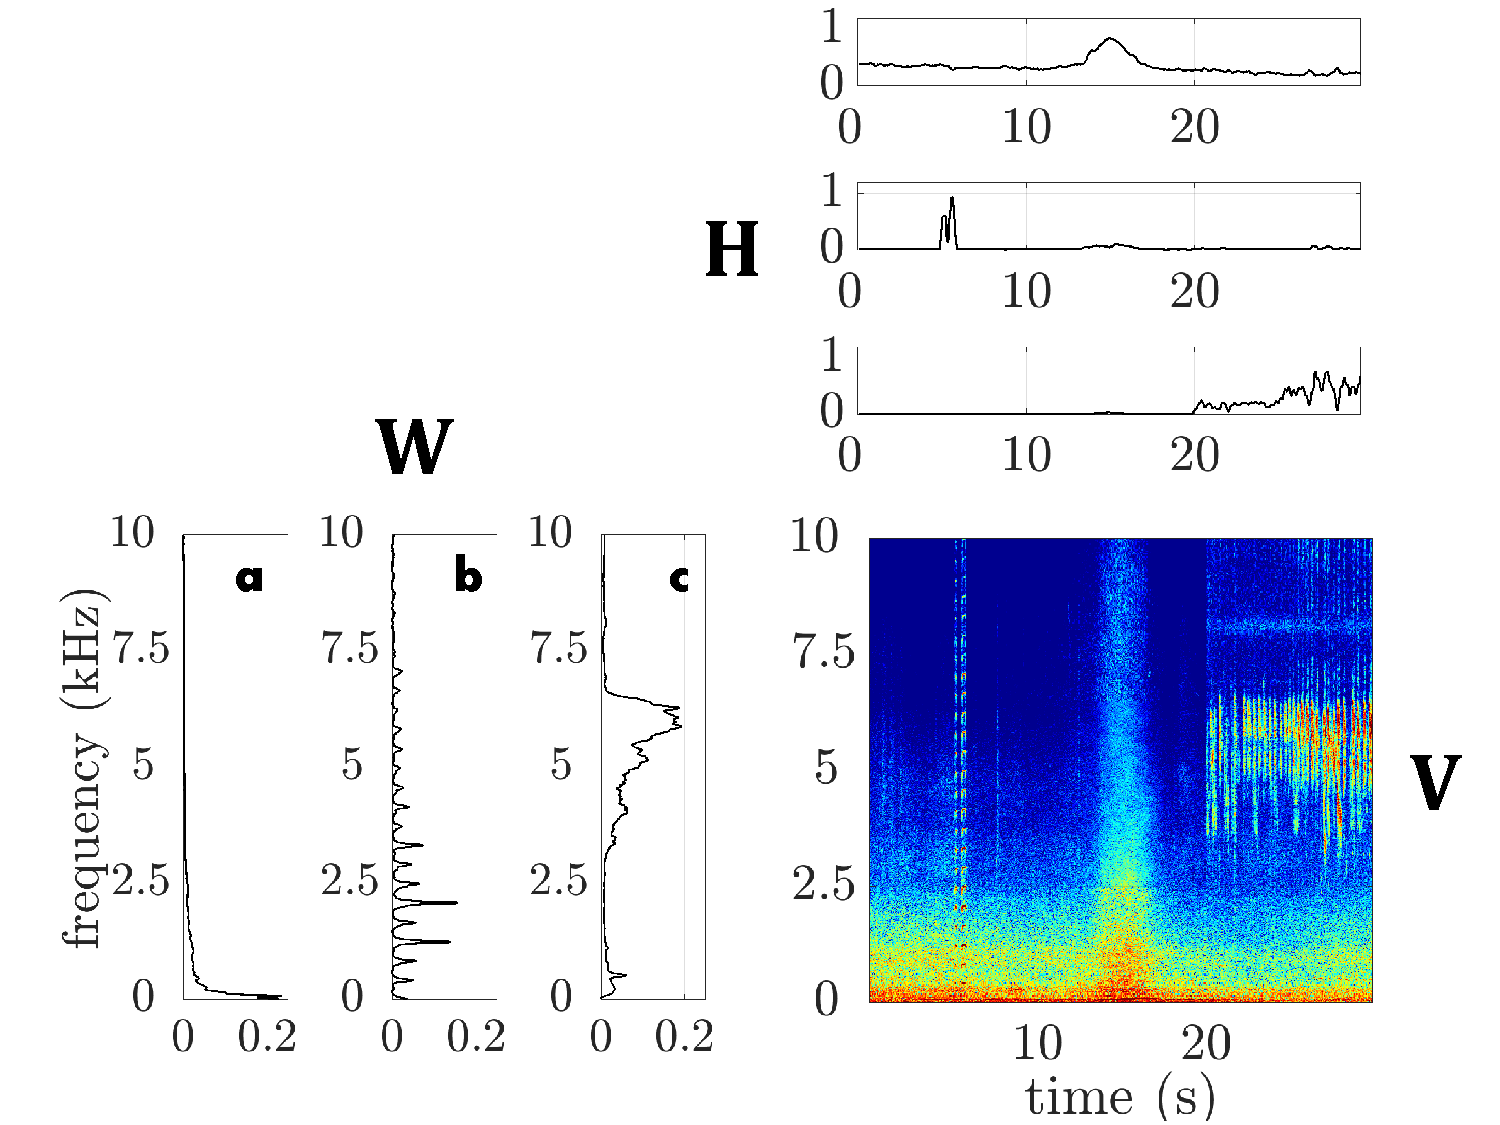
\includegraphics[width=.9\linewidth]{./figures/schema_introduction_nmf.pdf}
\caption{NMF decomposition of an audio spectrogram composed of 3 elements ($K$ = 3): passing car (a), car horn (b) and whistling bird (c).}
\label{fig:exampleNMF}
\end{figure}

The approximation of $\mathbf{V}$ by $\mathbf{WH}$ product is defined by a cost function to minimize,

\begin{equation}\label{eq:min-D-WH}
\underset{\mathbf{H} \geq 0, \mathbf{W} \geq 0}{\min} D\left(\mathbf{V} \Vert \mathbf{WH}\right),
\end{equation}

where $D(\bullet \Vert \bullet)$ is a divergence calculation such as:
\begin{equation}
D\left(\textbf{V} \vert\vert \mathbf{WH} \right) = \sum_{f = 1}^{F} \sum_{n = 1}^{N} d_{\beta}
\left(\textbf{V}_{fn} \vert \left[ \textbf{WH} \right]_{fn} \right).
\end{equation}

$d_{\beta}(x\vert y)$ is usually chosen as a $\beta$-divergence \cite{fevotte_algorithms_2011}, a sub-classes belonging to the Bregman divergences \cite{hennequin_beta-divergence_2011} which include 3 specific divergence calculations: the Euclidean distance (eq. \ref{eq:def_distEUC}), the Kullback-Leibler divergence (eq. \ref{eq:def_divKL}) and the Itakura-Sa\"{i}to divergence (eq. \ref{eq:def_divIS}):

\begin{subequations}\label{eq:divBetaGenerale}
\begin{numcases}{d_{\beta}(x\vert y) =}
    \frac{1}{2}(x-y)^2, & $\beta = 2$, \label{eq:def_distEUC}\\
    x\log \dfrac{x}{y} - x + y, & $\beta = 1$, \label{eq:def_divKL} \\
    \frac{x}{y} - \log \frac{x}{y} - 1 & $\beta = 0$. \label{eq:def_divIS}
\end{numcases}
\end{subequations}

The minimization problem (\ref{eq:min-D-WH}) is solved iteratively by updating the form of matrices $\mathbf{W}$ and $\mathbf{H}$. Different algorithms such as Alternating Least Square Method \cite{cichocki_regularized_2007} or Projected Gradient \cite{lin_projected_2007} have been considered. The most commonly used algorithm is the Multiplicative Update \cite{lee_algorithms_2000}. The latter method is chosen here, as it ensures non-negative results and the convergence of the results \cite{fevotte_algorithms_2011}.

\subsection{Supervised NMF}
The most easiest case of NMF is the one where the sound sources can be known \textit{a priori} and $\mathbf{W}$ can be built directly from audio samples. It leads to \textit{supervised} NMF (SUP-NMF). $\mathbf{H}$ is then the only matrix to estimate and is updated at every iteration (eq. \ref{eq:updateH}) \cite{fevotte_algorithms_2011}.

\begin{equation} \label{eq:updateH}
\textbf{H}^{(i+1)} \leftarrow \textbf{H}^{(i)}\otimes\left(\frac{\textbf{W}^T \left[\left(\textbf{WH}^{(i)} \right)^{(\beta-2)}\otimes\textbf{V} \right]}{\textbf{W}^T \left[\textbf{WH}^{(i)} \right]^{(\beta-1)}}\right)^{\gamma(\beta)}
\end{equation}

with $\gamma(\beta) = \frac{1}{2-\beta},$ for $\beta < 1$, $ \gamma(\beta) = 1$, for $\beta \in \left[1,2\right]$ and $\gamma(\beta) = \frac{1}{\beta-1}$ for $\beta > 2$. The product $A\otimes B$ and $A/B$ symbolized the Hadamard product and ratio.

Here, in an urban context, if the sound sources are known, their audio samples can be obtained to learn $\mathbf{W}$, see section \ref{part:dictionary_building}. As the position of each element is indexed, the traffic source separation from the other sound sources is made by extracting, from the dictionary and the activation matrix, the related elements:

\begin{equation}\label{eq:separationExtraction}
\mathbf{\tilde{V}}_{traffic} = \left[ \mathbf{WH} \right]_{traffic}.
\end{equation}

\subsection{Semi-supervised NMF}

The main issue with the supervised approach is the representational limit imposed by a fixed $\mathbf{W}$. To be completely successful, all the acoustical sources must be considered in it which is not possible in an urban environment. However, in our application setting, the main source of interest, \textit{i.e.} the traffic, can be known \textit{a priori} \ml{manque une phrase} semi-supervised NMF (SEM-NMF) \cite{lee_semi-supervised_2010} is considered to better take into account the interfering sound sources. To do so, $\mathbf{W}_{F \times (K+J)}$ is decomposed into two distinctive matrices: $\mathbf{W} = \left[ \mathbf{W_s}~\mathbf{W_r} \right]$ where $\mathbf{W_s}_{F \times K}$ is a fixed part of $\mathbf{W}$ composed of audio spectra and $ \mathbf{W_r}_{F \times J}$, a mobile part which is updated, see eq. \ref{eq:W_r_SS}. Thus it is possible to include elements not present in $\mathbf{W_s}$. The dimension of $\mathbf{W_r}$ is set up as $J << K$ in order to best considered the sound source present in $\mathbf{W_s}$. $\mathbf{H}$ is then also decomposed in two matrices, $\mathbf{H}_{(K+J) \times N} = \genfrac[]{0pt}{0}{\mathbf{H_s}}{\mathbf{H_r}}$. The eq. \ref{eq:nmf} becomes

\begin{equation}
\mathbf{V} \approx \mathbf{WH} = \mathbf{W_s H_s}+\mathbf{W_r H_r}.
\end{equation}

$\mathbf{H_r}$ and $\mathbf{H_s}$ are updated separately, see eq. \ref{eq:H_r_SS} \ref{eq:H_s_SS}.


{\scriptsize
\begin{subequations}\label{eq:WH-SSupdate}
\begin{align}
\mathbf{W_r}^{(i+1)} &\leftarrow \mathbf{W_r}^{(i)}\otimes\left(\frac{\left[\left(\mathbf{W_r H_r}^{(i)} \right)^{(\beta-2)}\otimes\mathbf{V} \right]\mathbf{H_r}^T}{\left(\mathbf{W_r H_r}^{(i)} \right)^{(\beta-1)}\mathbf{H_r}^T}\right)^{\gamma(\beta)}.\label{eq:W_r_SS}\\
\mathbf{H_r}^{(i+1)} &\leftarrow \mathbf{H_r}^{(i)}\otimes\left(\frac{\mathbf{W_r}^T \left[\left(\mathbf{W_r H_r}^{(i)} \right)^{(\beta-2)}\otimes\mathbf{V} \right]}{\mathbf{W_r}^T \left(\mathbf{W_r H_r}^{(i)} \right)^{(\beta-1)}}\right)^{\gamma(\beta)},\label{eq:H_r_SS}\\
\mathbf{H_s}^{(i+1)} &\leftarrow \mathbf{H_s}^{(i)}\otimes\left(\frac{\mathbf{W_s}^T \left[\left(\mathbf{W_s H_s}^{(i)} \right)^{(\beta-2)}\otimes\mathbf{V} \right]}{\mathbf{W_s}^T \left(\mathbf{W_s H_s}^{(i)} \right)^{(\beta-1)}}\right)^{\gamma(\beta)},\label{eq:H_s_SS}
\end{align}
\end{subequations}}

In this study, $\mathbf{W_s}$ is composed of traffic audio spectra to include in $\mathbf{W_r}$ all the other sources that can be present in the urban sound scenes. The traffic signal estimation is next defined by the fixed part,

\begin{equation}\label{eq:separationExtraction_SS}
\mathbf{\tilde{V}}_{traffic} = \left[ \mathbf{W_s H_s} \right].
\end{equation}

The addition of the mobile part $\mathbf{W_r}$ gives more flexibility. The representational capability is increased, thus the approach is more adaptive to the different urban sound environments. Applications of SEM-NMF can be found for musical \cite{weninger2012supervised, kitamura_music_2014} and speech content \cite{joder2012real, mysore2011non}.

\subsection{Thresholded Initialized NMF}\label{part:NMF_TI}

To allow even more flexibility while still considering prior knowledge of the source of interest, we propose a third approach based on the unsupervised NMF framework: Threshold Initialized NMF (TI-NMF). Usually, in unsupervised NMF, the dictionary is initiated randomly when there is no \textit{prior} knowledge on the sound sources present. Here, as the target sound source is known and the spectra are available, an initial dictionary, $\mathbf{W_0}$, is designed and then updated alternatively with $\mathbf{H}$,

\begin{equation}\label{eq:updateW_unsup}
\textbf{W}^{(i+1)} \leftarrow \mathbf{W}^{(i)}\otimes \left(\frac{\left[\left(\mathbf{W}^{(i)}\mathbf{H} \right)^{(\beta-2)}\otimes \mathbf{V} \right]\mathbf{H}^T}{\left[\mathbf{W}^{(i)}\mathbf{H} \right]^{(\beta-1)}\mathbf{H}^T}\right)^{\gamma(\beta)}.
\end{equation}

With this operation, $\mathbf{W_0}$ is oriented to the focused sound source (the road traffic) but also can be adapted to the content of the scene thanks to the updates. After $N$ iterations, each element $k$ of the final dictionary, $\mathbf{W'}$, is compared with its initial value in $\mathbf{W_0}$, in order to identify which element is stayed closed to the traffic component. A cosine similarity $D_{\theta}\left(\mathbf{W_0} \Vert \mathbf{W'} \right)$ is computed for each element $k$ as it is an invariant scale and a bounded method,

\begin{equation}
D_{\theta}\left(\mathbf{w_0} \Vert \mathbf{w'} \right) = \frac{\mathbf{w_0}.\mathbf{w'}}{\Vert \mathbf{w_0}  \Vert . \Vert \mathbf{w'} \Vert}.
\end{equation}

where $\mathbf{w}$ is a $k$ element of $\mathbf{W}$ of $F \times 1$ dimension. When $D_{\theta}\left(\mathbf{w_0} \Vert \mathbf{w'} \right)$=1, the element $k$ from $\mathbf{W'}$ is equal to the in $\mathbf{W_0}$ \ml{pas clair, a quoi sert le k ?}. If $D_{\theta}\left(\mathbf{w_0} \Vert \mathbf{w'} \right)$=0, the element is fully different. Next, the similarities are sorted in descending order \ml{le sort n'est pas necessaire, le seuil suffit}. The extraction of traffic elements in $\mathbf{W'}$ is carried out by a hard thresholding method \cite{donoho1994threshold}. It consists in weighting in a binary way the traffic elements $\mathbf{W'}$ according to $D_{\theta}\left(\mathbf{w_0} \Vert \mathbf{w'} \right)$ and a threshold value such as:

\ml{on pourrait tout a fait imaginer l'ajout d'élément de dictionaire random pour se rapprocher de la semi.}

\begin{equation}
\mathbf{w}_{traffic} = \alpha_k \mathbf{w'}.
\end{equation}
with
\begin{subequations}\label{eq:WH-TIupdateHard}
\begin{numcases}{\alpha_k =}
1  & iff \quad $D_{\theta}\left(\mathbf{w}_{0} \Vert \mathbf{w'} \right) > t_h$, \\
 0 & else.
\end{numcases}
\end{subequations}

\ml{faire un par resumant les prop des trois methodes avec un accent sur l'utilisation de la connaissance a priori.}

These methods are applied on simulated sound scenes in order to compare the estimated sound levels with a non ambiguous reference. In \cite{gloaguen2018Estimation}, the sound corpus was composed of a mix of traffic samples with specific sound classes (\textit{alert, animals, climate, human, mechanics, transportation}). Here, in order to implement this method in embedded sensors, a new and more realistic sound corpus by considering more realistic urban sound environments with many kind of sound sources.

\section{Design of realistic urban sound scenes}\label{part:urban_scene}

\ml{Il faut faire une figure et un paragraphe resumant la figure. Voici un essai (je pense d'ailleurs que cela devrait faire partie des claims dans l'intro) : In order to validate the above described methods, the evaluation corpus is both required to be realistic and non ambiguous in terms of traffic sound level. The former calls for the use recordings of urban sound environments, and the latter imposes the use of controled use of sound sources with known properties: onset and offset time location, and volume. Indeed, the precise annotation of the sound level of a given source of interest in a polyphonic mixture is not feasible. We thus propose to design such evalution corpus based on two corpora. The first, called the reference corpus, is a set of recordings of urban sound environments, from which a sort of "score" is extracted manually, \textit{i.e.} which sound source is present from this time to this time, at which sound level. The second, called the elemental corpus, is a set of monophonic recordings of sound sources that are occurs in the scenes of the reference. The recordings of the elemental corpus are not taken from the reference corpus. The evaluation corpus is then built by sequencing recordings of the elemental corpus according to the scores of the reference corpus. (Le reste est a reecrire avec les termes proposés)}

More precisely, the urban sound scenes are taken from 76 recordings from 2 to 5 min, achieved in the \nth{13} district of Paris (France) at 19 different locations \footnote{Recordings were made as part of the Grafic project funded by Ademe}, which cover four various sound environments (Figure \ref{fig:map_grafic}), see Figure \ref{fig:map_grafic}. A complete description of the experimental protocol can be found in \cite{aumond_modelling_2017}. Two of the 76 recordings are rejected for the analysis because the audio files were corrupted, resulting in 74 valid audio files assumed as representative of the variety of sound environments. The recordings are listened and categorized within four different sound environments, as proposed in \cite{can_describing_2015}: park (P, 8 audio files with a cumulative duration of 16min01), quiet street (Q, 33 audio files with a cumulative duration of 77min27), noisy street (N, 24 audio files with a cumulative duration of 56min10) and very noisy street (vN, 9 audio files with a cumulative duration of 21min42). Then, each audio file is annotated, annotating the start, end time \ml{and level ?} of each sound event along with its sound class. \ml{cette phrase ne dis probablement pas ce qsue tu veux dire annotation et Transcription sont des termes equivalents, The aim of the annotation phase is next to transcribe the recordings}, in order to obtain simulated sound scenes with the same \ml{ca peut preter a confusion en implicitant une distribution statistique : distribution} of sound events as the recordings and therefore as close as possible to the realistic scenes.

\begin{figure}[t]
\centering
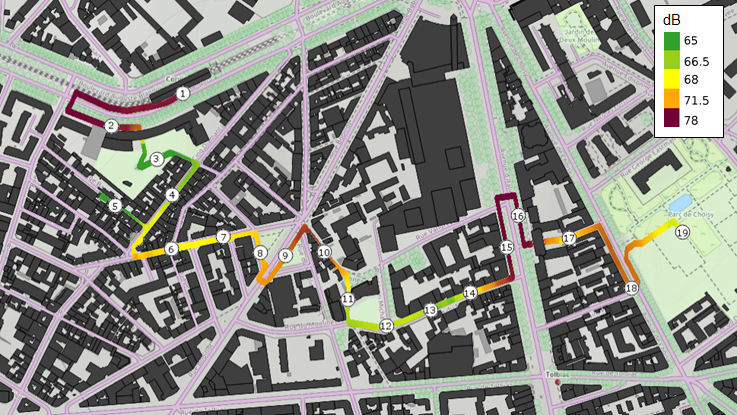
\includegraphics[width=\linewidth]{./figures/trajet_19pts.png}
\caption{Walked path with the 19 stop points  \cite{aumond_modelling_2017}.}
\label{fig:map_grafic}
\end{figure}


\subsection{Generation of the evaluation corpus}\label{part:simScene}
The sound scenes are generated with the \textit{SimScene} software\footnote{Open-source project available at: \url{https://bitbucket.org/mlagrange/simscene}}, \cite{rossignol_simscene:_2015}, which is a simulation software generating monaural sound mixtures in wav format with a 44.1 kHz sampling rate from an isolated sound database.
This software have already been used in a wide range of experiments for sound detection algorithm assessment \cite{lafay_new_2014, benetos2016detection}. \ml{Pas clair The control of high level parameters can be handled by the user as the sound class occurence, the time between each sample of one sound class, the ratio between the sound level of an event class with the background (i.e the \textit{event background ratio} shorten \textit{ebr})\dots Each parameter is completed with a standard deviation to bring random behavior. It allows too the design of a sound mixture from an annotation text file. A remplacer par ceci: The \textit{SimScene} software allows for several type of sequencing, from abstract ones (time indexes and amplitudes are drawn from random distributions) to  precise ones, where the time indexes and amplitudes for each event is set by the user. The latter type is considered in this study.}
As output, \textit{SimScene} generates an audio of the global sound mixture and an audio for each sound class present in the scene, which makes it possible to know their exact contributions in the scene, see Figure \ref{fig:example_simScene}.

\begin{figure}[t]
    \centering
       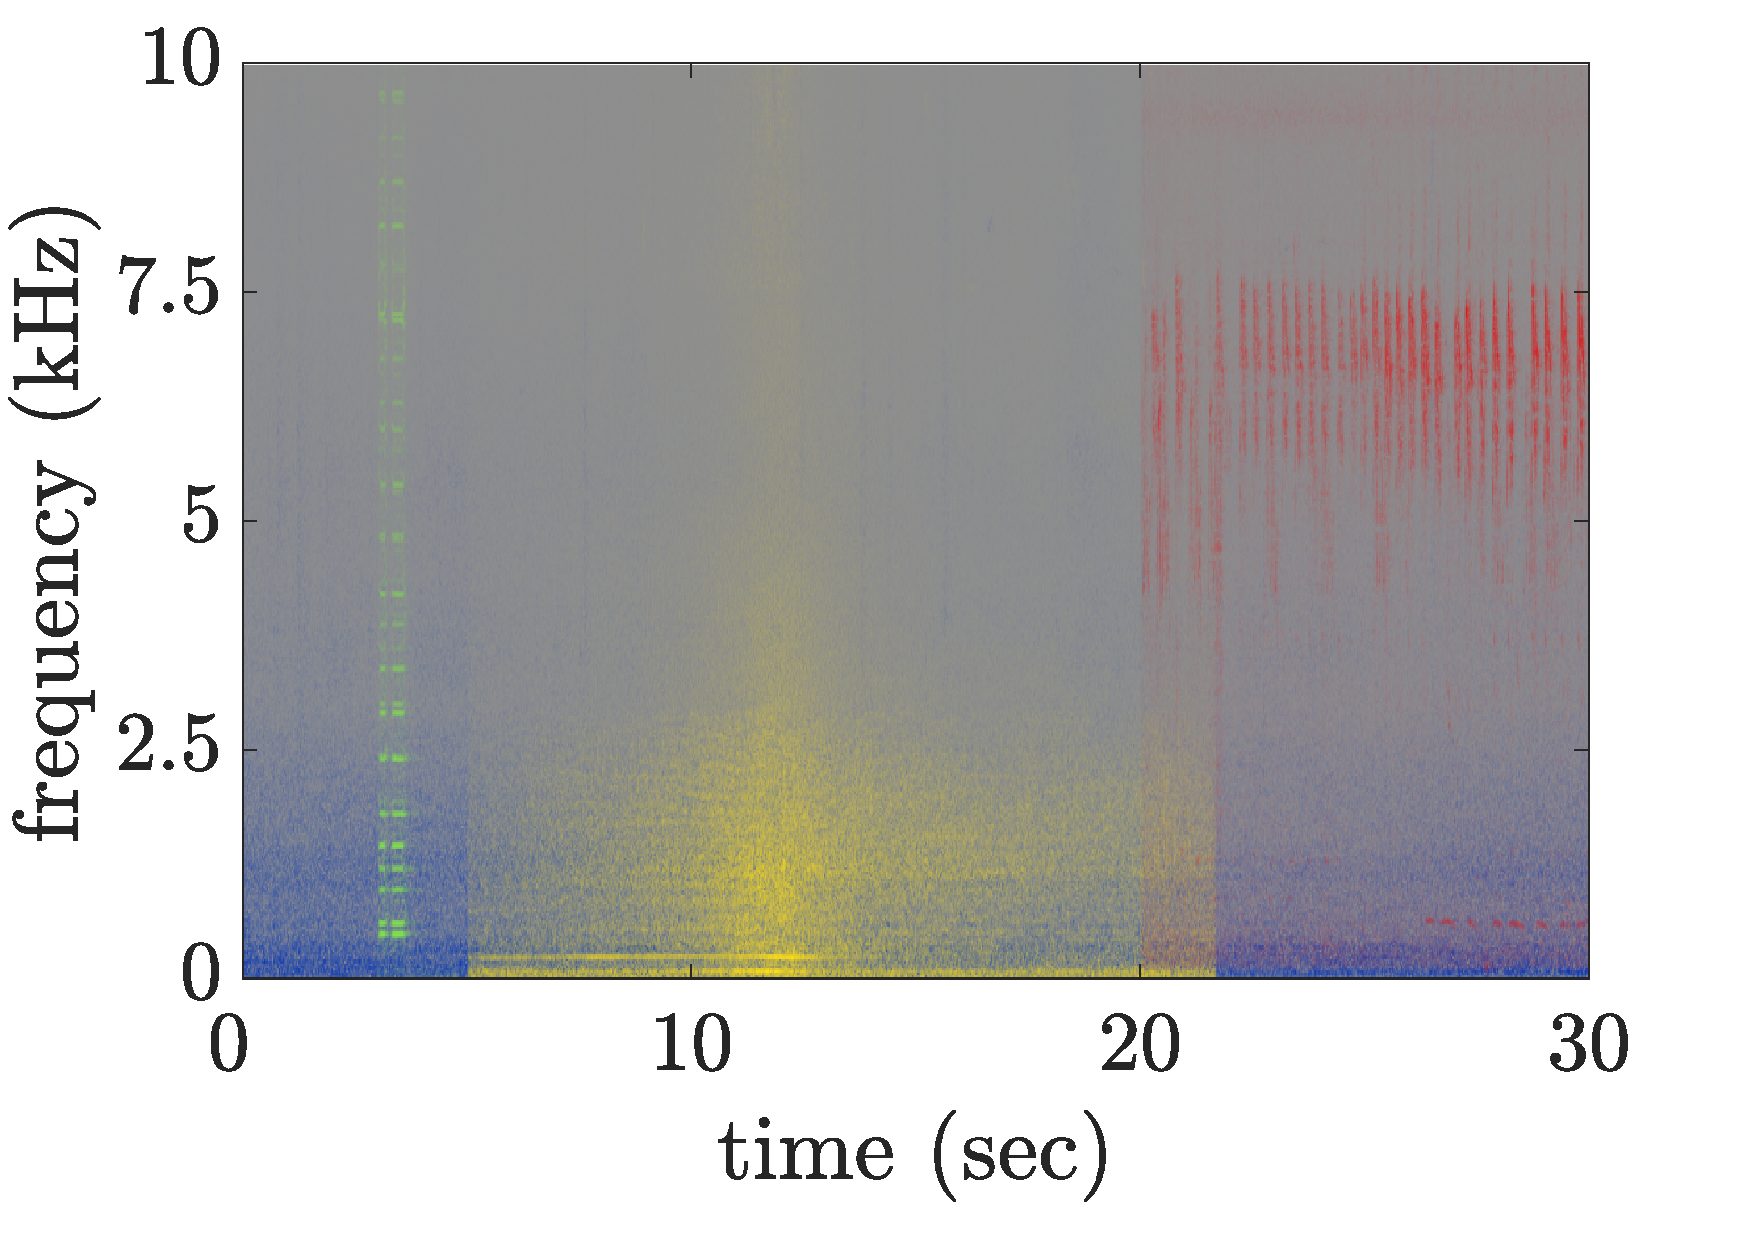
\includegraphics[width=.8\linewidth]{./figures/exampleSimScene.pdf}
    \caption{Spectrogram of a simple scene created with the \textit{SimScene} software with a sound background (road traffic in green) and 3 sound events (car horn in purple, passing car in red and whistling bird in blue).}
    \label{fig:example_simScene}
\end{figure}

To transcribe the recordings in simulated scenes, a high quality sound database (wav format, 44.1 kHz sampling rate, high \textit{Signal Noise Ratio}) has been built-up from audio samples found online (\textit{freesound.org}) or with the help of an already existing sound database \cite{salamon2014dataset}. The sound database is composed of two categories of sound: the \textit{event} category, which includes 245 brief sound samples considered as salient, with a 1 to 20 seconds duration and classified among 21 sound classes (\textit{ringing bell, whistling bird, car horn, passing car, hammer, barking dog, siren, footstep, metallic noise, voice \dots}) and the \textit{background} (or \textit{texture}) category gathering 154 long duration sounds ($\approx$ 1m30), whose acoustic properties do not vary in time. This category includes among others\textit{whistling bird, crowd noise, rain, children playing in schoolyard, constant traffic noise} \dots sound classes. Each sound class is composed of multiple samples (\textit{carHorn01.wav, carHorn02.wav \dots}) that are randomly chosen by the \textit{simScene} software to bring diversity.
As the road traffic is the main component in urban environment and is the sound source of interest, recordings of car passages has been made on the Ifsttar's runway. The recordings has been made for 4 cars (Renault Scenic, Renault M\'egane, Renault Clio and Dacia Sandero),  at different speeds and gear ratios. Overall, 103 car passages have been recorded. \ml{ajouter une description sur les problématiques d'overfitting et de generalisation. Cela doit etre un rappel d'un texte ecrit dans la partie nmf. A ce titre, cela pourrait etre une extension de l'etude, on en reparle} The audio samples of the first two cars (Renault Scenic and Renault M\'egane) are included in the \textit{SimScene}'s sound database (50 audio files in total). The last 53 audio samples are dedicated to the dictionary design as part of NMF, see section \ref{part:dictionary_building}. A full description of the recordings can be found in \cite{gloaguen_creation_2017}.

\begin{table}[t]
\centering
\caption{$mTIR$ for each sound environment.\ml{les captions doivent etre self-contained, pas d'acronymes non evident}}
\begin{tabular}{lc}
 & $mTIR$ (dB)\\ \hline
 park & -9.10 ($\pm$ 7.35) \\
 quiet street & 0.88 ($\pm$ 5.92) \\
 noisy street & 6.96 ($\pm$ 5.16) \\
 very noisy street & 15.75 ($\pm$ 9.78) \\ \hline
\end{tabular}
\label{tab:mTIR}
\end{table}

With this built-up database, the \textit{SimScene} software and the annotations of the recordings, 74 simulated sound scenes are generated, which have the temporal structure of the reference recordings. The \textit{ebr} parameter is adjusted manually on each sound scene to be faithful compared to the recorded scenes. To validate this adjustment, the mean \textit{Traffic Interfering Ratio} is calculated and summarized on Table \ref{tab:mTIR}. It expresses, on all the scenes of an sound environment, the mean difference between the equivalent traffic sound levels of each scene, $L_{p,traffic}$, with the sound level of the \textit{interfering} sound class, $L_{p, interfering}$, which gathered all the other sound sources not related to the traffic, see Eq \ref{eq:mTIR}. It quantifies the predominance of the traffic component for the 4 types of sound environments.

\begin{equation}\label{eq:mTIR}
mTIR = \frac{\sum_{i = 1}^M L_{p,traffic} - L_{p, interfering}}{M}.
\end{equation}

As it is the sound environment where the traffic is less present, the $mTIR$ is always negative for the \textit{park}. The \textit{interfering} sound class is therefore the main sound source. In the case of the \textit{quiet street}, the $TIR$ can be positive or negative depending on the traffic presence on the scene. For the 2 others sound environments, when the traffic become the main sound source, $mTIR$ is always positive.

\subsection{Perceptual test}

To evaluate the level of realism of the corpus of transcribed urban sound scenes, a perceptual test is considered.

The perceptual test is conducted with a panel of 50 subjects that are asked to assess the level of realism on a 7-point scale (1 is \textit{not realistic at all}, 7 is \textit{very realistic}) of a set of transcribed and recorded scenes. The total number of sound scenes tested is set at 40. The first half includes 20 30-seconds audio files, including 5 scenes that belong to the sound environment \textit{park}, 6 from \textit{quiet street}, 4 from \textit{noisy street} and 5 from \textit{very noisy street} chosen randomly among the recorded scenes. The second half is composed of the transcribed scenes coresponding to the 20 reference scenes. In order to limit the duration of the test to preserve the concentration of the subjects, each subject listens to only a subset of 20 sound scenes. All the scenes are normalized to the same sound level, chosen at 65 dB, and the subjects are not allowed to change the output sound level once set at the beginning of the experiment.

The experimental design is elaborated following a partially Balanced Incomplete Block Design (PBIBD) \cite{john1977optimal} that determines the listening order of each participant based on fixed parameters (number of listeners, total number of audio, number of audio assessed by each listeners). The listening order is then built in a such way than each listener listens the same amount of recorded scenes and transcribed scenes to avoide statistical biais. The experimental design and the listening order per participant are performed with the package \textit{sensoMineR} on the \textit{R} software \cite{le_sensominer:_2008}.\\

The test was available online on the 8 February 2017 and the needed number of participant has been reached 12 days later. During the test, the participants had the possibility to listen to each scene as many times as wanted before assessing, without being able to change their judgment afterwards. The participants could also leave a comment on each audio to explain the rating \footnote{The interface of the experiment is available \url{http://soundthings.org/research/xpRealism}}. Based on the information provided, the panel of 50 listeners was made of 31 males and 18 females (one not documented) with an average age of 36 ($\pm$ 12) years old. $62\%$ of the participants declared having no experience in the listening of urban sound mixtures. Figure \ref{fig:boxPlot_test} summarizes the score distributions of all the listeners for the recorded (rec.) and the transcribed (trans.) scenes.

\begin{figure}[t]
\centering
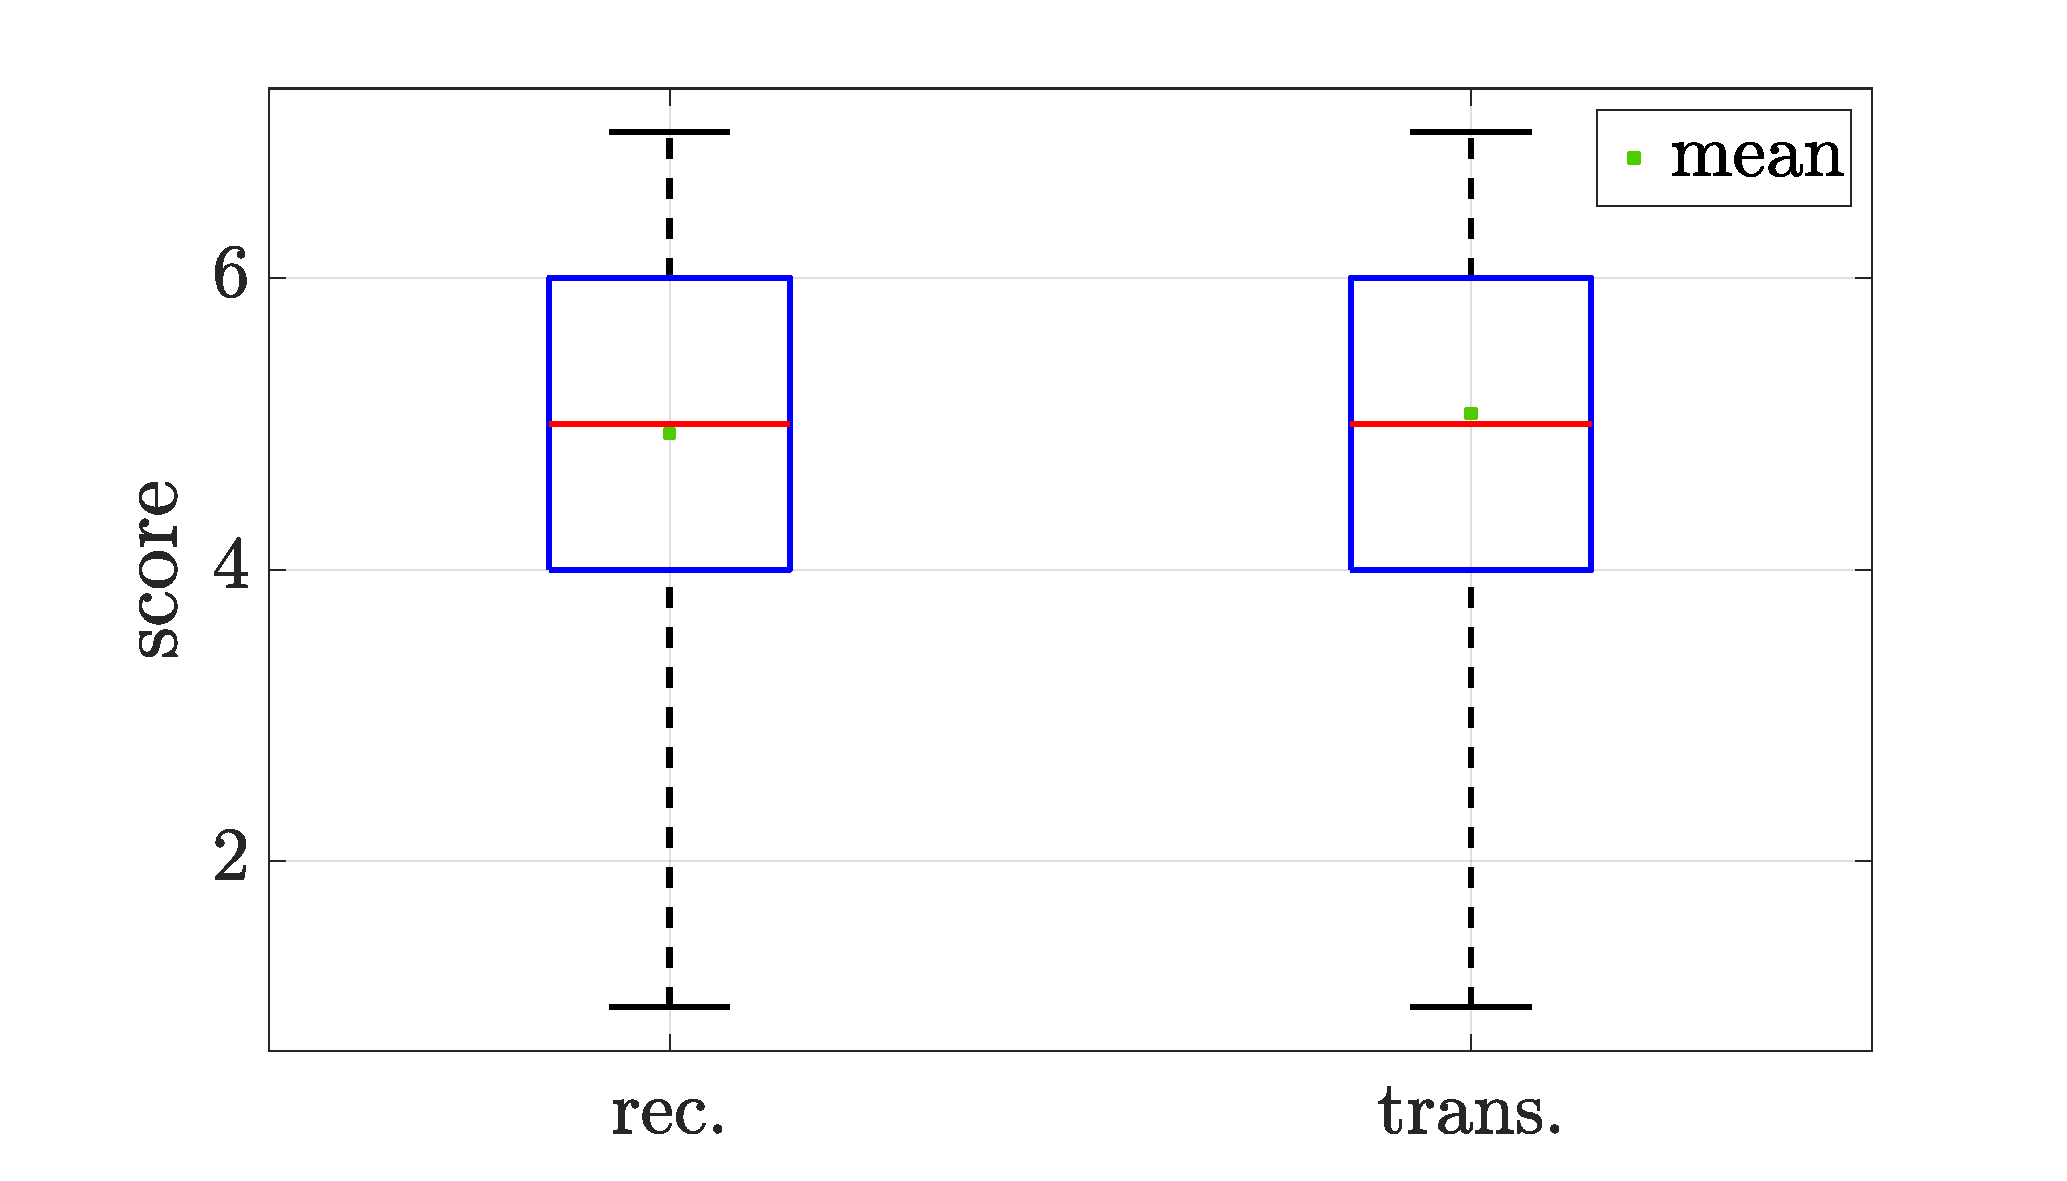
\includegraphics[width=\linewidth]{figures/testPerceptif_boxplotType_EN.pdf}
\caption{Box and whiskers plot of the rating of realism according to the type (recorded /transcribed). \ml{Il faut tout expliciter, as tu vraiment besoin de toutes ces informations ?}}
\label{fig:boxPlot_test}
\end{figure}

The distributions of the notations according to the type are extremely similar. The mean score for the transcribed scenes is even superior to the recorded ones ($m_{trans.}$ = 5.1 ($\pm 1.6$), $m_{rec}$ = 4.9 ($\pm 1.6$)). These results confirm that the recorded and the transcribed scenes are perceived in a similar way by the panel. More details on the results can be found in  \cite{gloaguen_creation_2017}.

\ml{ce serait quand meme bien d'avoir un test stat, au moins un ttest}

As the transcribed sound corpus is sufficiently close to the recordings, these sound mixtures can be used to assess the performances of NMF to estimate the traffic sound level.

\section{Experimental protocol}\label{part:expProtocol}

The design of the experiment aims at evaluating in a meaningful manner the performance of the different systems. To do so, the 74 sound scenes, organized on 4 different types of sound environments are iteratively fed to the processing system which output an estimate of the equivalent sound level of the traffic within each scene $\tilde{L}_{p, traffic}$ (dB). This result is then compared to the reference sound level value given by the simulation process, $L_{p,traffic}$, see Figure \ref{fig:bloc_diagram_estimator}.

\begin{figure}[t]
\centering
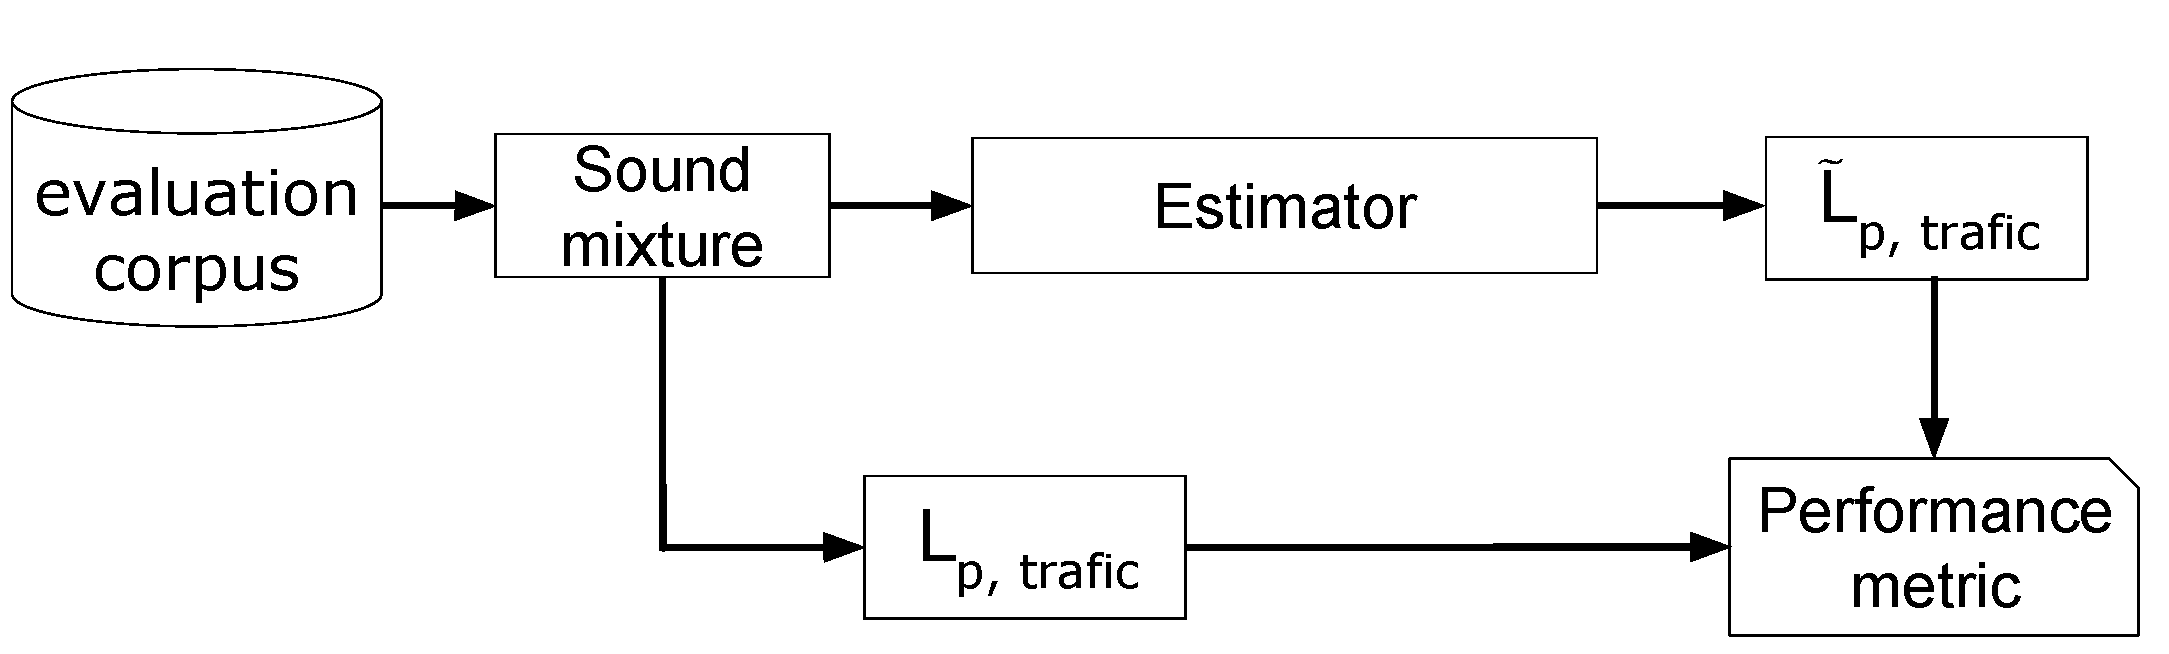
\includegraphics[width=.9\linewidth]{figures/bloc_diagram_estimator.pdf}
\caption{Bloc diagram of the experimental protocol.}
\label{fig:bloc_diagram_estimator}
\end{figure}

\subsection{Metrics}

The traffic sound levels, $\tilde{L}_{p,traffic}$, are compared to the exact values, $L_{p,traffic}$, through the Mean Absolute Error ($MAE$) \cite{willmott2005advantages}. The $MAE$ expresses the quality of the long-term reconstruction of the signal and consists in the average of the absolute difference between the exact and the estimated sound levels,

\begin{equation}
MAE = \frac{\sum_{i = 1}^{M} \vert L_{p,traffic}^i - \tilde{L}_{p,traffic}^i \vert}{M}.
\end{equation}

It is then possible to express the $MAE$ error for each unique setting but, also, to average this metric according to the 4 sound environments to be able to estimate the optimal setting that offers the lowest error for all the sound environments:

\begin{equation}
mMAE = \frac{\sum_{i = 1}^4 MAE_i}{4},
\end{equation}

where the other experimental factors (method, $f_c$, $\mathbf{K}$, $\mathbf{w_t}$, $\beta$, threshold value $\mathbf{t_h}$) are fixed.


\begin{figure*}[t]
\centering
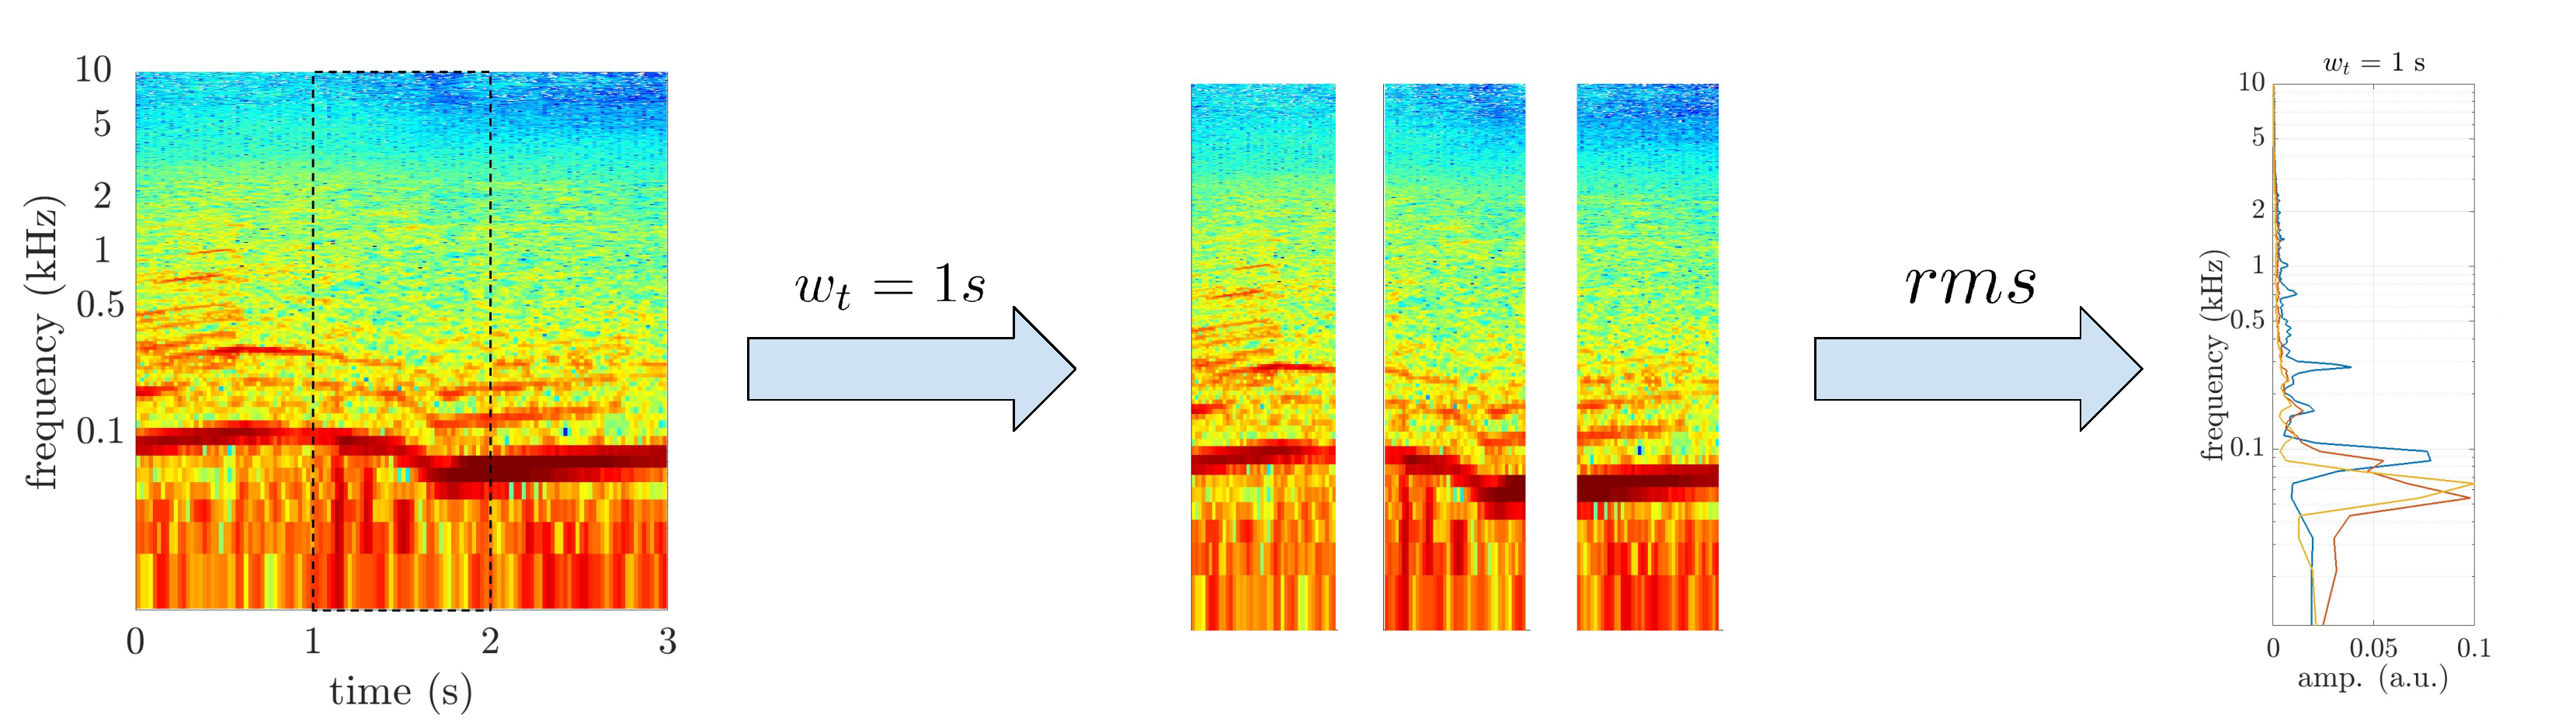
\includegraphics[width=0.8\linewidth]{figures/extractionDictionary2.pdf}
\caption{Dictionary building on a 3 second example of a passing car with $w_t = 1$ second. In this case, the dictionary $\mathbf{W}$ is made of 3 spectra, each representative of a texture frame of $w_t$ duration.}
\label{fig:example_dictionary}
\end{figure*}

\subsection{Methods}

As the road traffic is mainly composed of a low frequency content, a frequency low-pass filter (LP filter) is considered as baseline. It consists in filtering the sound scenes at different cut-off frequencies $f_c \in \lbrace$500, 1, 2k, 5k, 10k, 20k$\rbrace$ Hz. The remaining energy located in the pass-band is assimilated to road traffic,

\begin{equation}
\mathbf{\tilde{V}}_{traffic} = \mathbf{V}_{f_c}.
\end{equation}

The second estimator is based on the three NMF formula presented in part \ref{part:nmf} (see Figure \ref{fig:bloc_diagram_nmf}). Multiple experimental factors take part in these cases where each of them having different modalities.

\begin{figure}[t]
\centering
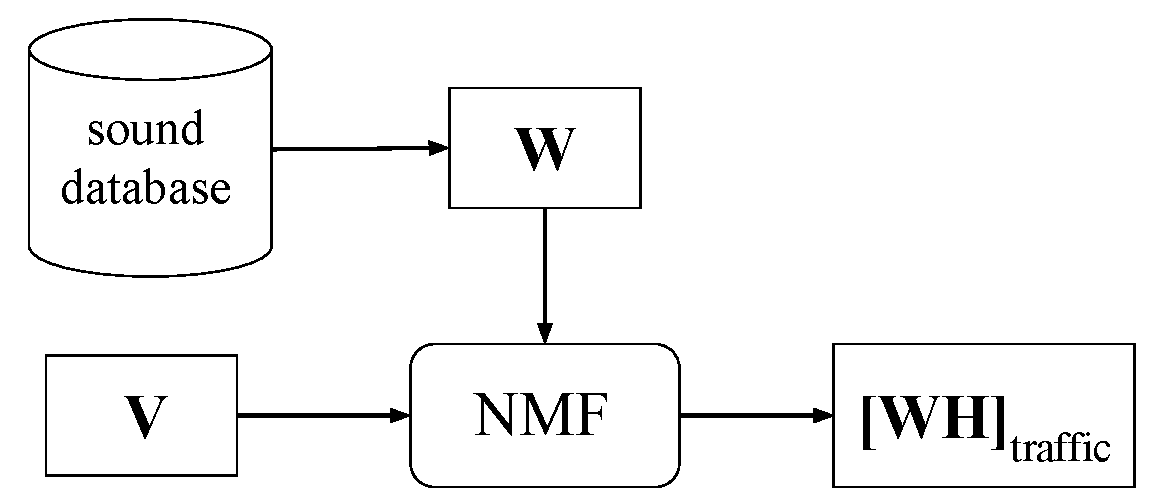
\includegraphics[width=.9\linewidth]{figures/bloc_diagram_NMF_EN_2.pdf}
\caption{Bloc diagram of the NMF estimator.}
\label{fig:bloc_diagram_nmf}
\end{figure}

\subsection{Dictionary building for NMF methods}\label{part:dictionary_building}

The dictionary is designed from a second sound database specially dedicated to this task to prevent any overfitting issues. It contains  53 audio files of the 2 cars (Dacia Sandero and Renault Clio) recorded on the runway, see part \ref{part:simScene}. Those recordings have not been considered for the creation of the evaluation dataset.

First the spectrogram of each audio file is computed (window $w = 2^{12}$ with 50 $\%$ overlap). The spectrogram is then cut in multiple temporal frames of $w_t  = \lbrace$0.5, 1$\rbrace$ second duration. In each cut spectrogram, the root mean square on each frequency bin is calculated to obtained a spectrum of $F \times 1$ dimension. This method allows the description of the audio sample with finer spectra and then having the different characteristic pitches of the traffic spectra. An illustrative example on a 3 seconds sample is displayed in Figure \ref{fig:example_dictionary}. From the 53 audio files, we obtain respectively for $\mathbf{w_t}\in$ $\lbrace$0.5, 1$\rbrace$ second, 2218 and 1109 elements.

A $\mathbf{K}$-means clustering algorithm is applied to reduce these dimensions to $\mathbf{K} \in \lbrace$25, 50, 100, 200$\rbrace$ in order to avoid redundant information and decrease the computation time. The resulting $\mathbf{K}$ centroids are taken as the elements of $\mathbf{W}$. \ml{Vraiment utile ? Furthermore, the case where each audio generates one spectrum from its spectrogram is added ($\mathbf{w_t} = all$). In this case, the dictionary elements are based on the spectral envelope of the audio samples. With only 53 audio samples, the number of elements in $\mathbf{W}$ with the $\mathbf{K}$-mean clustering algorithm is reduced to $\mathbf{K} \in \lbrace$25, 50$\rbrace$.}

The obtained dictionary is expressed in third octave bands to decrease the dimensionality. \ml{Citer ou enlever, A previous experimental validation revealed that the use of third octave bands does not impact the performances of the chosen estimator in this study.}  Each basis of $\mathbf{W}$ is then normalized as $ \Vert \mathbf{w}_k \Vert = 1$ where $\Vert \bullet \Vert$ is the $\ell_1$ norm. Table \ref{tab:experimental_factorsNMF} summarizes the different modalities of the two experimental factors ($\mathbf{K}$ and $\mathbf{w_t}$).

\subsection{NMF experimental factors}

NMF is performed for 3 $\beta$-divergences: $\beta$ = 2 (euclidean distance), $\beta$ = 1 (Kullback-Leibler divergence) and $\beta = 0$ (Itakura-Sa\"ito divergence). The spectrogram $\mathbf{V}$ and the dictionary $\mathbf{W}$ are represented in a logarithmic scale through a third band octave representation that reduces the high frequency predominance where the traffic component is absent. In addition, as the number of frequency bins is reduced ($F$ = 29), the computation time is reduced too. 400 iterations are performed to get a stabilized results. For SEM-NMF, the number of elements in $\mathbf{W_r}$ is set to $J = 2$. For hard thresholding, the threshold value, $\mathbf{t_h}$ is set between 0.30 and 0.60 with a 0.01 increment.
Each unique association of modalities between each experimental factor forms an experimental setting. For the filter estimator, 24 settings are computed (4 $\times$ 6). For SUP and SEM-NMF, 240 settings are computed (4 $\times$ 2 $\times$ (2 $\times$ 4 + 1 $\times$ 2) $\times$ 3). Finally, for TI-NMF, the number of settings is much higher (3720) due to the higher cardinality of the set of threshold values (4 $\times$ 1 $\times$ (2 $\times$ 4 + 1 $\times$ 2) $\times$ 3 $\times$ 31).
The experimental factors and their different modalities are displayed on Tables \ref{tab:experimental_factorsFilter} and \ref{tab:experimental_factorsNMF}.

The approximated traffic spectrograms $\mathbf{\tilde{V}}_{traffic}$ are obtained after 400 iterations. The estimated traffic sound level in dB, $\tilde{L}_{p, traffic}$, is then computed,

\begin{equation}
\tilde{L}_{p, traffic} = 20\log_{10}\frac{p_{rms}}{p_0},
\end{equation}

where $p_0$ is the reference sound pressure, $p_0 = 2\times 10^{-5}$ Pa. For each setting, $M$ traffic sound levels, corresponding to the $M$ scenes of each sound environment, are then calculated.

\begin{table*}[t]
\caption{Experimental factors and their modalities for the frequency low-pass filter baseline estimator.}
\centering
\begin{tabularx}{17.5cm}{L{3cm}@{}C{12cm}@{}C{2cm}@{}}
	\hline
    \textbf{\begin{tabular}[c]{@{}l@{}}experimental \\ factors\end{tabular}} & \textbf{modalities} & \begin{tabular}[c]{@{}C{2cm}@{}}\textbf{number of}\\ \textbf{modalities}\end{tabular}\\ \toprule
\end{tabularx}

\begin{tabularx}{17.5cm}{L{3cm}@{}@{}C{3cm}@{}@{}C{3cm}@{}@{}C{3cm}@{}@{}C{3cm}@{}C{2cm}@{}}
    \textbf{sound environment} & park & quiet street & noisy street & very noisy street & 4 \\
\end{tabularx}

\begin{tabularx}{17.5cm}{L{3cm}@{}@{}C{2cm}@{}@{}C{2cm}@{}@{}C{2cm}@{}@{}C{2cm}@{}@{}C{2cm}@{}@{}C{2cm}@{}C{2cm}@{}}
\rowcolor[HTML]{C0C0C0}
   $\mathbf{f_c}$ (kHz) & 0.5 & 1 & 2 &  5 & 10 & 20 & 6\\
   \bottomrule
\end{tabularx}

\label{tab:experimental_factorsFilter}
\end{table*}


\begin{table*}[t]
\centering
\caption{Experimental factors and their modalities for the NMF estimator.}
\begin{tabularx}{17.5cm}{L{3cm}@{}C{12cm}@{}C{2cm}@{}}
	\hline
    \textbf{\begin{tabular}[c]{@{}l@{}}experimental \\ factors\end{tabular}} & \textbf{modalities} & \begin{tabular}[c]{@{}C{2cm}@{}}\textbf{number of}\\ \textbf{modalities}\end{tabular}\\ \toprule
\end{tabularx}

\begin{tabularx}{17.5cm}{L{3cm}@{}C{3cm}@{}@{}C{3cm}@{}@{}C{3cm}@{}@{}C{3cm}@{}C{2cm}@{}}
    \textbf{sound environment} & park & quiet street & noisy street & very noisy street & 4\\
\end{tabularx}

\begin{tabularx}{17.5cm}{L{3cm}@{}C{4cm}@{}@{}@{}C{4cm}@{}@{}C{4cm}@{}C{2cm}@{}}
	\rowcolor[HTML]{C0C0C0}
  \textbf{method} & SUP NMF & SEM NMF & TI NMF & 3\\
\end{tabularx}

\begin{tabularx}{17.5cm}{L{3cm}@{}C{4cm}@{}@{}C{4cm}@{}@{}C{4cm}@{}C{2cm}@{}}
    $\mathbf{w_t}$ (s)& 0.5 & 1 & \textit{all} & 3 \\
\end{tabularx}

\begin{tabularx}{17.5cm}{L{3cm}@{}C{3cm}@{}@{}C{3cm}@{}@{}C{3cm}@{}@{}C{3cm}@{}C{2cm}@{}}
	\rowcolor[HTML]{C0C0C0}
    $\mathbf{K}$ & 25 & 50 & 100 & 200 & 4\\
\end{tabularx}


\begin{tabularx}{17.5cm}{L{3cm}@{}C{4cm}@{}@{}C{4cm}@{}@{}C{4cm}@{}C{2cm}@{}}
   $\mathbf{\beta}$ & 0 & 1 & 2 & 3\\
\end{tabularx}

\begin{tabularx}{17.5cm}{L{3cm}@{}C{12cm}@{}C{2cm}@{}}
	\rowcolor[HTML]{C0C0C0}
   hard threshold $\mathbf{t_h}$ & from 0.30 to 0.60 with a 0.01 step & 31\\
   \bottomrule
\end{tabularx}
\label{tab:experimental_factorsNMF}
\end{table*}


\section{Results and discussion}\label{part:results}

Table \ref{tab:results} summarizes the lowest $mMAE$ errors according to the method (LP filter, SUP-NMF, SEM-NMF and TI-NMF) and $\beta$ with the others corresponding modalities.

\begin{table*}[t]
\centering
\caption{Best $mMAE$ errors according to the experimental factors $\beta$ and \textit{method} (in bold letter, the lowest error).}
\begin{tabular}{@{}ccccccc@{}}
\toprule
\textbf{method} & $f_c$ (kHz) & $\mathbf{\beta}$ & $\mathbf{K}$ & $\mathbf{w_t}$ (s) &  $\mathbf{t_h}$ &  \textbf{$mMAE$} (dB) \\ \midrule
filter & 20 & - & - & - & - & 3.76 ($\pm$ 4.35) \\
filter & 0.5 & - & - & - & - & 2.14 ($\pm$ 1.83) \\
\hline \hline
SUP-NMF & - & 0 & 200 & 0.5 & - & 4.06 ($\pm$ 4.69) \\
SUP-NMF & - & 1 & 200 & 0.5 & - & 2.79 ($\pm$ 3.38) \\
SUP-NMF & - & 2 & 25 & 1 & - & 2.32  ($\pm$ 2.80) \\
\hline \hline
SEM-NMF & - & 0 & 200 & 1 & - & 2.05 ($\pm$ 0.70) \\
SEM-NMF & - & 1 & 200 & 1 & - & 1.94 ($\pm$ 0.38) \\
SEM-NMF & - & 2 & 200 & 1 & - & 2.39 ($\pm$ 1.23) \\
\hline \hline
TI-NMF & - & 0 & 25 & 1 & 0.39 & 1.42 ($\pm$ 0.89)\\
TI-NMF & - & 1 & 100 & 1 & 0.35 & 1.38 ($\pm$ 0.88)\\
\textbf{TI-NMF }& - & \textbf{2} & \textbf{200} & \textbf{0.5} & \textbf{0.32} & \textbf{1.24 ($\pm$ 1.24)}\\
\bottomrule
\end{tabular}
\label{tab:results}
\end{table*}

The LP filter with $f_c = 20$ kHz cut-off frequency is equivalent to considerate the sound level of the entire scene without specific distinction between the sound sources. The error is then important with a high standard deviation ($mMAE =$ 3.76 ($\pm$ 4.35) dB). The lowest error for a LP filter is obtained with $f_c$ = 500 Hz ($mMAE =$ 2.14 ($\pm$ 1.83) dB). \ml{It allows a balance between the discarded and remaining energy through the sound environments.}

When considering all the sound scenes, SUP-NMF does not succeed to achieve a lower error than the 500 Hz LP filter for all the $\beta$ values. By adding the mobile part $\mathbf{W_r}$ in the dictionary, SEM-NMF with $\beta = 0$ and $\beta = 1$ allows a lower error than 500 Hz LP filter with a reduced standard deviation especially for $\beta = 1$ ($mMAE = 1.94$ ($\pm$ 0.38) dB).

TI-NMF is the approach with the lowest global error ($<$ 1.50 dB). The best result is obtained for TI-NMF ($MAE$ = 1.24 ($\pm$ 1.24) dB) with $\beta = 2$, $\mathbf{K}$ = 200, $\mathbf{w_t}$ = 0.5 s and as threshold value $\mathbf{t_h}$ = 0.32. This combination of settings offers the most fitted method to be adapted to all the sound environments.
Furthermore, on the dictionary creation, except SEM-NMF where all the best methods according to $\beta$ use the same dictionary, no specific dictionary form through all the method, is used. SUP and SEM-NMF privilege a high number of element ($\mathbf{K}$ = 200) with a fine description of the audio samples ($\mathbf{w_t} \in \lbrace 0.5$,$1 \rbrace$ second). For TI-NMF, the composition of the initial dictionary is more diverse both on the $\mathbf{K}$ value and on the finesse  of the description ($\mathbf{w_t} \in \lbrace all$,$0.5 \rbrace$ second).

From these global results, the $MAE$ errors are compared to the LP filter and each method for the 4 types of sound environments, see Figure \ref{fig:mae_env}.

\begin{figure}[t]
\centering
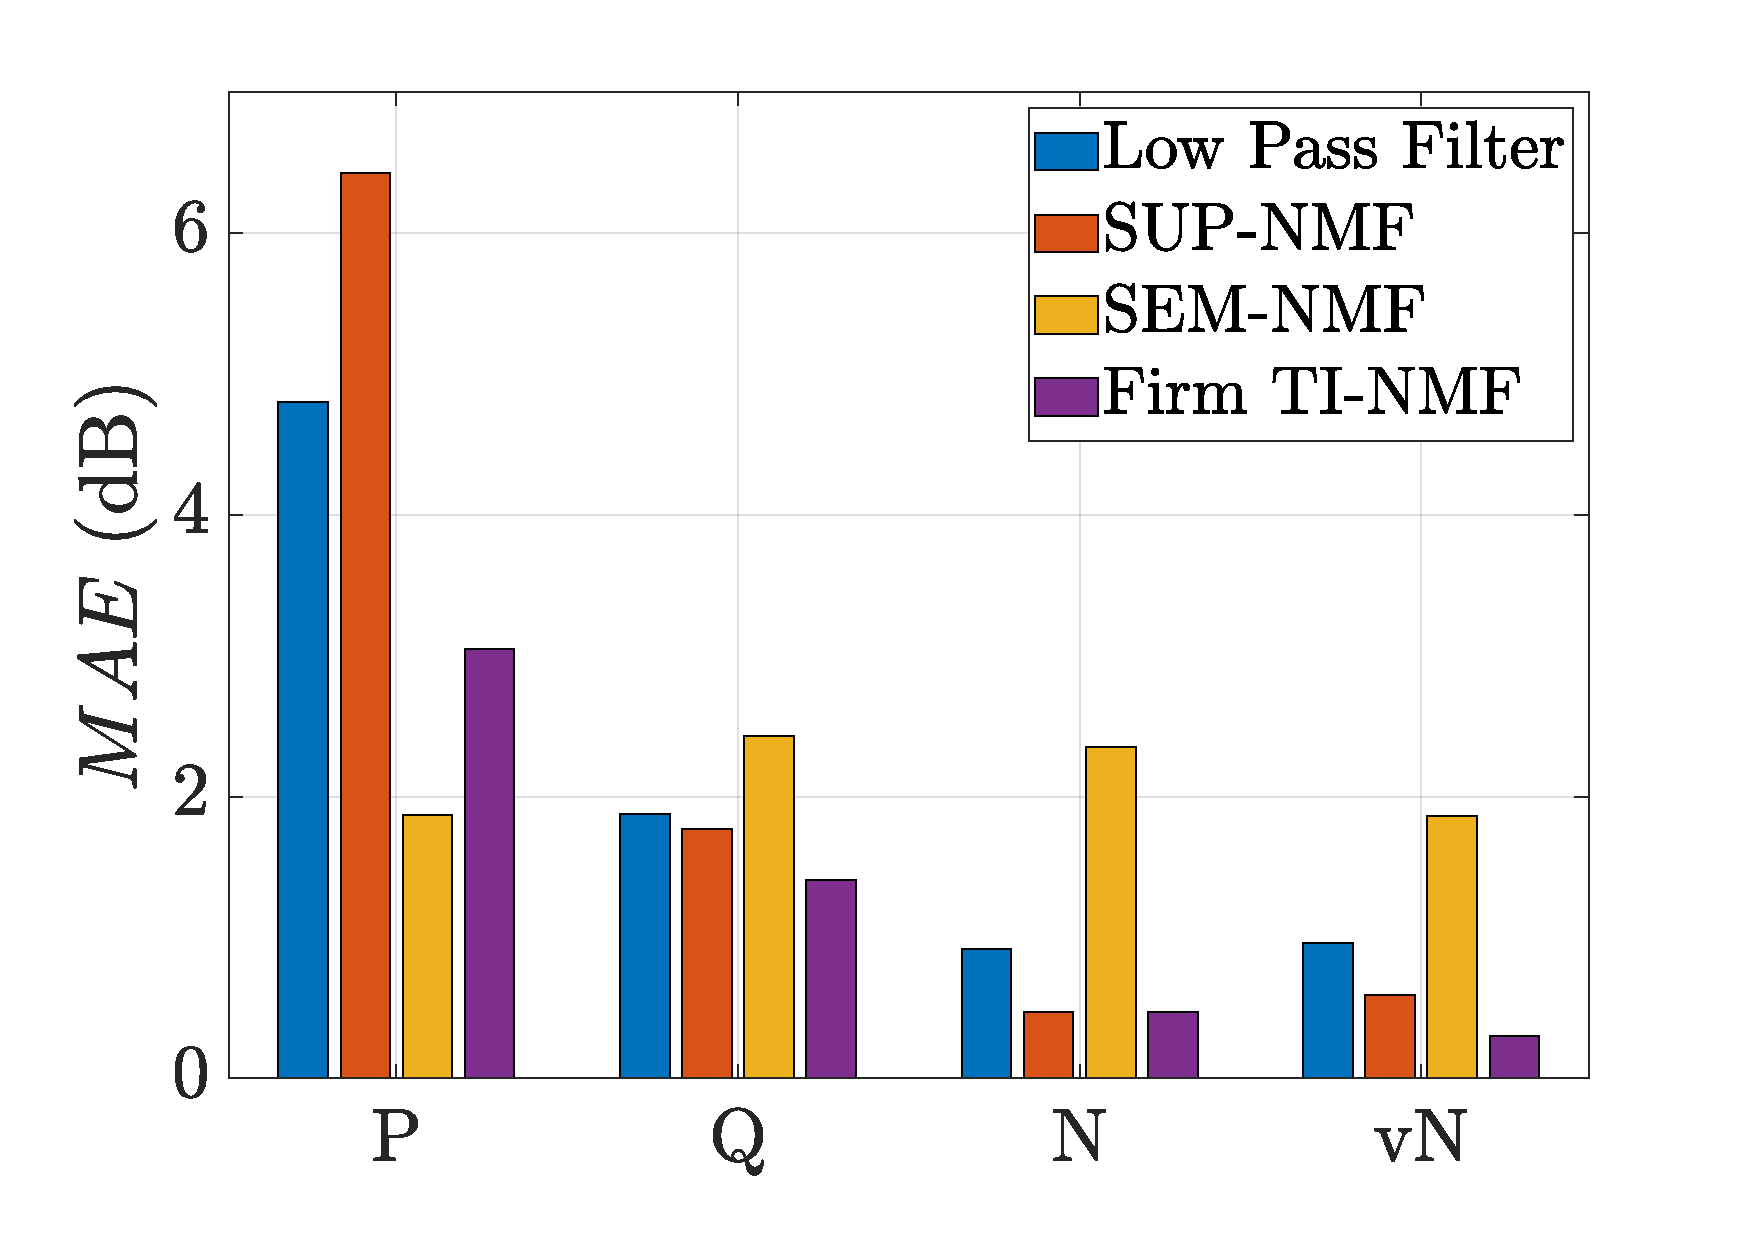
\includegraphics[width=\linewidth]{figures/mea_grafic_bar.pdf}
\caption{$MAE$ errors according to each sound environment for the best combination of the LP filter ($f_c$ = 500 Hz), SUP-NMF ($\beta$ = 2, $\mathbf{K}$ = 25, $\mathbf{w_t}$ = 1 second), SEM-NMF ($\beta$ = 1, $\mathbf{K}$ = 200, $\mathbf{w_t}$ = 1 second) and TI-NMF ($\beta$ = 2, $\mathbf{K}$ = 200, $\mathbf{w_t}$ = 0.5 second, $\mathbf{t_{h}} = 0.32$).}
\label{fig:mae_env}
\end{figure}

Aside SEM-NMF, all the methods show the same error evolution the same error evolution: a decrease of the error with the increase of the traffic predominance. On contrary, SEM-NMF show an almost constant error for all 4 sound environments. The LP filter error is mainly important for environments where the traffic is less present. As this approach considers the remaining energy as the traffic component, no distinction is made between the different sound sources not related to the traffic component. In the opposite, for noisy and very noisy environments, the performances of the LP filter are good ($MAE$ $<$ 1 dB). The errors are then due to a high deletion of the traffic energy by the filter while it becomes the main sound source.

Despite a fixed dictionary composed of traffic spectra, SUP-NMF fails to identify correctly the traffic component particularly for \textit{park} ($MAE$ = 6.42 dB) environments. With this method, as NMF minimizes the cost function, eq. \ref{eq:min-D-WH}, the dictionary's elements are used to model the other sound sources. In the opposite, for \textit{noisy} and \textit{very noisy} environments, SUP-NMF identifies correctly the traffic components ($MAE$ $<$ 0.6 dB) as it is the main source.
In the case of SEM-NMF, adding the mobile dictionary, $\mathbf{W_r}$, makes it possible to include the other sound sources not present in the dictionary. If this behavior is advantageous for the \textit{park} environment ($MAE$ = 2.10 dB) where lot of different kind of sources are present, it is less advantageous for the rest of the environments where the traffic becomes predominant resulting in the highest errors. Indeed, this degree of freedom generates higher error as $\mathbf{W_r}$ is not constrained and is free to include traffic component in it, penalizing the traffic sound level estimation.

\ml{Pas clair, enlever ? : Besides having the lowest $mMAE$ error, TI-NMF presents the most performing results. The park environment is the only case where an other NMF approach out-performed TI-NMF ($MAE$ = 2.95 dB). In this sound environment, the traffic dictionary is then composed, in average, of more than half the 200 elements in $\mathbf{W'}$ (136 elements). For the rest of the sound environments, TI-NMF has the lowest error. For very noisy environment the error is even very low ($MAE=$ 0.28 dB). In this case, in average, $\mathbf{W'}$ is composed of 198 traffic elements. This method out-performed SUP-NMF since, as $\mathbf{W_0}$ is updated, the final dictionary $\mathbf{W'}$ is then most suited to the sound scene than a fixed dictionary.}

Considering a unique dictionary fitted to the sound scene under evaluation thus makes TI-NMF very effective when traffic is predominant while, by the use of the thresholding, it discards the elements of the dictionary that deviated too much when the traffic is less present.

\section{Conclusion}

The non-negative matrix factorization framework has been considered as a source separation tool to estimate the traffic sound level  from a corpus of urban sound scenes artificially built. Those scenes are designed to be as similar as possible to the outputs of a deployed sensor networks with the advantages of the simulation process (sound level and position of each source controlled and known). The realism of the scenes has been verified thanks to a perceptual test.

The results confirm the potential of the NMF method on such application scenario as it takes into account the overlap between the multiple sound sources present in cities and is suited to monophonic sensor networks. Different NMF algorithmic schemes have been studied through the supervised and semi-supervised approach. On all the sound environments, these common approaches reveal to be not sufficiently efficient: supervised NMF approach, with its fixed dictionary, does not succeed to estimate correctly the traffic sound level especially when this sound source is quiet, while semi-supervised approach with the presence of a mobile part in the dictionary is the best estimator for \textit{park} environments but fails on heavily traffic scenes.

The proposed approach, named Thresholded Initialized NMF, achieved the lowest error in the evaluation corpus. Consequently, in the case where the location or the type of sound environments the sensors are monitoring cannot be identified (for instance within a mobile measurement framework), TI-NMF appears to be the method of choice. If the sound environment can be identified through a prior analysis, or based on positioning data \cite{can2015noise,lavandier2016urban}, it should be possible to adapt the estimation procedure by selecting the most efficient approach in order to further reduce the error in the estimated road traffic sound levels.

Further analyses are required to extend the proposed method to other sound sources, such as birds or voices sounds, which can conveniently be done by replacing or adding elements in the dictionary. This would prove useful in the context of muti-source noise mapping that is  gaining interest \cite{aumond2017Probabilistic, aletta2015soundscape}. Finally, the selected parameters stand for the corpus of sound mixtures of this study. Further analyses on various corpus of sound scenes are needed to evaluate the robustness of the method, and select the most relevant approaches for specific sound environments (predominance of water or industrial sounds, rural environments \dots).

For reproducibility purposes, the evaluation corpus, the experimental protocol and the programs developed under the Matlab software are available online \footnote{\url{https://github.com/jean-remyGloaguen/articleApplied2018}}. %This study proposes also a realistic urban sound corpus that could be greatly appreciate for research communities dedicated to the detection, identification or source separation tasks.


\section*{References}
\bibliographystyle{elsarticle-num}
\bibliography{bibliographie_applied}

\end{document}
